\section{Overview of Direction Finding}
In this section, an analysis is made of different the direction finding techniques which exist. The most applicable of these will be examined in more details following.
Classical methods of direction finding algorithms \cite{tuncer2009classical}.
\begin{itemize}
	\item Beamforming: by introducing the correct phase delay to each channel of the array, the array factor can be made to be such that the signal in quesetion is added coherently by each element of the array.
		This phase delay indicates the direction of arrival of the signal. The coherent addition of the signals allows for much higher SNR. 
\end{itemize}

\section{Direction Finding Techniques}
A Radio Direction Finder \gls{rdf} is a passive device able to ascertain the direction of a source of electromagnetic radiation which occurs in the RF frequency range, often defined as between \SI{3}{\kilo\hertz} and \SI{300}{\giga\hertz}. 

The general structure of a direction finding system is an antenna array connected to a receiver connected to a processing module connected to a display providing output to operators.

Radio DF has been around since the start of the 1900's. Some of the first people to work on DF  systems were Marconi and Brown. One of the first systems developed by them was a device to locate the bearing from shore to a ship which was broadcasting a signal. Their device was used by manually rotated a two-element array with half-wavelength spacing to and monitoring the amplitude of the output of the antenna.

(Move this later): As discussed in \cite{farrier1990direction}, many high-performance DF algorithms which have been proposed over the years have had stringent requirements for array geometry or signal environment. The requirement for this project is for the system to be versatile and reconfigurable, so no such restrictions on array geometry or signal environment or modeling accuracy must exist. 

\subsection{Classes of Direction Finder Systems}
The following overview of types of direction finding systems is based on discussions in the Electronic Warfare and Radar Systems Engineering Handbook \cite{center2012electronic}.
In general, classes of system include:

\subsection{Scanned beam}
This is a direct amplitude technique. An antenna with gain (non-uniform beam) is rotated and this causes the power output of the antenna to vary with rotation angle. This is the earliest form of direction radio direction finding and was implemented in the early 1900's. 
One of the first uses of this RDF device was to in a system developed by Marconi locate the bearing to a ship which was transmitting a signal for navigation purposes. A loop antenna was frequently used in the early 1900's as it was a simple antenna to construct and the beam pattern has a sharp null. 
An example antenna and beam pattern are shown in \autoref{fig:lit_loop_antenna}. As the change in antenna output power per degree rotated is highest around the null, the antenna was often aligned such that the signal of interest was in the null. 
If multiple signals originating from different bearings are present, the system cannot operate. 
While today it may be possible to put highly selective receivers on the output of the antenna, this technology did not exist when scanning beam DF systems were originally used.

Note that as the beam pattern is symmetric about both the x and y axis, there are in general 4 ambiguous points. However, if the antenna can be rotated such that the signal is in the null, there is then only 2 ambiguous points, or \SI{180}{\degree} ambiguity. This can be resolved with an  additional antenna element to resolve. Note also that this is not an instantaneous DF technique as it requires time for the antenna to be rotated. Hence, this technique is not suitable for finding transients. 

Loop antennas DF systems are very sensitive to multipath errors, especially ionospheric reflection \cite{jenkins1991smallaperture}. 
\begin{figure}
  \centering
  \begin{subfigure}[b]{0.48\textwidth}
    \centering
    \includegraphics[width=0.8\textwidth]{lit_review/loop_antenna}
    \caption{Loop antenna used for direction finding in 1918. Src: \cite{grabau1989funkpeiltechnik}}
  \end{subfigure}
  ~
  \begin{subfigure}[b]{0.48\textwidth}
    \centering
   \includegraphics[width=0.7\textwidth]{lit_review/loop_antenna_beam}
   \caption{Beam pattern of loop antenna or dipole. Note the sharp null. Src: \cite{jenkins1991smallaperture}}
  \end{subfigure}
  \caption{Loop antenna and beam pattern}
  \label{fig:lit_loop_antenna}
\end{figure}

\subsection{Crossed Loop}
The crossed loop technique is an amplitude comparison technique. 
As is shown in \autoref{fig:lit_crossed_loop_antenna}, using two loop antennas perpendicular to one another produces two beam patterns: one being proportional to the sine of the angle and the other to the cos of the angle. 
By comparing the signal power from each antenna, it is possible to ascertain the \gls{aoa}. This system is instantaneous as only a single pulse is necessary to ascertain the ratio of antenna output power. However it has many ambiguities. Some ambiguities can be resolved with a sense antenna. 
For optimal ambiguity resolution, the crossed loop should be rotated such that signal of interest is located in the null of one of the loops and the peak of the other. This resolves ambiguity but at the expense of the system not being real-time.
As with the scanned beam, the crossed loop suffers from significant performance degradation arising from multipath, specifically ionospheric reflection. 
In the 1930's a marine radio direction finder network using the crossed loop amplitude comparison technique was set up for marine navigation. Then, during World War II, rapid improvements to RDF technology were made with the operating frequency of the systems being extended into the VHF and UHF band  and extensive RDF networks being installed \cite{jenkins1991smallaperture}.
\begin{figure}
  \centering
  \begin{subfigure}[b]{0.3\textwidth}
    \includegraphics[width=\textwidth]{./img/lit_review/loop_antenna_crossed}
    \caption{Example of crossed loop antenna.}
  \end{subfigure}
  ~
  \begin{subfigure}[b]{0.4\textwidth}
    \includegraphics[width=\textwidth]{./img/lit_review/loop_antenna_crossed_beam}
    \caption{Crossed loop antenna beam pattern showing difference in magnitude seen by each loop. Src: \cite{jenkins1991smallaperture}}
  \end{subfigure}
  \caption{Crossed loop antenna and beam pattern}
  \label{fig:lit_crossed_loop_antenna}
\end{figure}

\subsection{Adcock Array}
The Adcock array was developed and patented in 1919 by British army engineer Frank Adcock \cite{gething1991radio}.
Instead of using loop antennas, the Adcock array makes use of two orthogonally orientated (crossed) pairs of monopole or dipole antennas. Typically a North-South pair and an East-West pair are used. These antenna pairs produce the same beam pattern as the loop antennas. 
As a loop antenna can be modeled by two vertical antennas on the sides and two horizontal antennas on the top and bottom of the loop, it should be clear that the loop is not polarisation selective. While the direct beam from the signal source may be vertically polarised, the reflected beam from atmospheric reflection was also being received and corrupting the signal output of the array.
The Adcock array which uses only vertical elements maintains the same beam pattern as the loop but is not sensitive to horizontally polarised radiation hence offers better performance for a DF system.
The antenna configuration of Adcock and Watson-Watt is shown in \autoref{fig:lit_adcock_array}.
This array configuration was studied extensively in the 1930's and played a significant role in the electronic warefare of World War II \cite{gething1991radio}.

\begin{figure}
  \centering
  \begin{subfigure}[b]{0.25\textwidth}
    \includegraphics[width=\textwidth]{./img/lit_review/adcock_model}
  \end{subfigure}
  ~
  \begin{subfigure}[b]{0.6\textwidth}
    \includegraphics[width=\textwidth]{./img/lit_review/adcock_implementation}
  \end{subfigure}
  \caption{Left: model for adcock antenna showing N-S and E-W pairs. Right: Japanese implementation of array for 2 MHz direction finding. Src: \cite{japanesecommunications}}
  \label{fig:lit_adcock_array}
\end{figure}


\subsection{Watson-Watt Evaluation}
Ambiguity and multipath are one of the major difficulties which need to be overcome in direction finding systems. 
In the mid 1920s, Sir Robert Watson-Wat developed an improved DF system based on the Adcock array configuration. This is an amplitude comparison technique. 
As discussed above, the beam pattern of the output of an Adcock array is one cosine shaped beam and one sine shaped beam. By exploiting the trigonometric properties of these functions and adding an additional sense element, Watson-Watt developed a method to compute the angle of arrival from an array with this cos/sin property. 
This evaluation technique showed significant improvement in rejection of ionospheric reflections and made ambiguity resolution easier.

The mathematics around this technique will not be explored in detail here, but a graphical view of the antenna and receiver structure can be seen in \autoref{fig:watson-watt}.
For a more detailed discussion of the mathematics behind the Watson-Watt DF algorithm, see Poisel \cite{poisel2008introduction}. For a simulation of Watson-Watt algorithm as well as a discussion around an ambiguity resolution implementation using a sense antenna see: \cite{adcockwatsonwattrdf}.

\begin{figure}
  \centering
  \begin{subfigure}[b]{0.48\textwidth}
    \includegraphics[width=\textwidth]{./img/lit_review/watson-watt-processing-analogue}
    \caption{View showing transformer configuration to produced required difference signals. Src: \cite{poisel2008introduction}}
  \end{subfigure}
  ~
  \begin{subfigure}[b]{0.48\textwidth}
    \includegraphics[width=\textwidth]{./img/lit_review/watson-watt-processing-digital}
    \caption{Abstraced view of signal chain for digital processing. Src: \cite{rhode2000introtodf}}
  \end{subfigure}
  \caption{Watson-Watt array processing technique using the Adcock array. Note that difference channels from crossed beams are formed}
  \label{fig:watson-watt}
\end{figure}

\subsection{Doppler}
By the principle of Doppler shift, moving an antenna towards a signal source increases the observed frequency while moving an antenna away from a source lowers the observed frequency. 
If an antenna is rotated around a central point (tracing out the circumference of a circle), there will be 
The Doppler shift is given by: \cite{poisel2012electronic}
\begin{equation}
  \Delta f = \frac{B\omega}{c}f_c\sin(\Uppsi)
\end{equation}
Where \(B\) is the length of the antenna baseline, \(\omega\) is the angular velocity of the antenna, \(f_c\) is the carrier frequency of the signal source and \(\Uppsi\) is instantaneous difference between the angle towards the signal source and the angle of the rotating antenna (this is shown graphically in \autoref{fig:lit-review-doppler-switching}. By rotating one antenna around a reference antenna and measuring the received signal frequency difference, the Doppler shift can be measured and with the above equation the AoA calculated.

However, As discussed by Jenkins, to DF a \SI{100}{\mega\hertz} tone with a Doppler shift of \SI{3}{\mega\hertz}, the antenna would need to be rotated with a tangential velocity of \SI{10000}{\metre\per\second} \cite{jenkins1991smallaperture}. 
It is not practical to rotate an antenna at such a high speed. 
Hence, rather than physically rotating an antenna, what is done in practice is that a Doppler shift is synthesised by rapidly switching between sampling different elements of a large circular array. 
Typically between 12 and 30 elements are used for Doppler DF arrays. 
Also graphically in \autoref{fig:lit-review-doppler-switching} is this typical implementation of a Doppler DF system using antenna switching.

As discussed by Jenkins \cite{jenkins1991smallaperture}, Doppler is not a high accuracy system due to the signal distortion introduced by switching the sampled antenna. Furthermore, Doppler DF is not suited to locating transients for two reasons:
\begin{enumerate}
  \item it is not an instantaneous technique due to there being some time required to switch between sampling all of the antennas. For example, a typically time required to switch between all elements of an array may be \SI{6}{\milli\second} \cite{rhode2000introtodf}. This is unsuitable for transients which may last only a few hundred nanoseconds.
  \item it generally needs a narrow-band signal which has a well defined carrier frequency so that the Doppler shift is well defined. Impulsive transients do not have this characteristic.
\end{enumerate}

For a more detailed discussion of the mathematics behind Doppler DF, see the Rhode \& Schwarz report \cite{rhode2000introtodf}. 
\begin{figure}
  \centering
  \begin{subfigure}[b]{0.48\textwidth}
    \centering
    \includegraphics[width=\textwidth]{./img/lit_review/doppler-2-antenna}
    ~ 
    \caption{Model for Antenna 2 rotating around stationary Antenna 1 with angular velocity \(\omega\). Src: \cite{poisel2012electronic}}
  \end{subfigure}
  ~
  \begin{subfigure}[b]{0.48\textwidth}
    \centering
    \includegraphics[width=0.6\textwidth]{./img/lit_review/doppler-switching}
    \caption{Practical implementation switching antennas for pseudo-Doppler DF system. Src: \cite{jenkins1991smallaperture}}
  \end{subfigure}
  \caption{Model for Doppler DF system}
  \label{fig:lit-review-doppler-switching}
\end{figure}


\subsection{Time Difference of Arrival}
\gls{tdoa} is a DF system which is typically used for finding of impulsive sources; sources which emit a pulse that exists for a short time duration where the pulse has a clearly defined start and end. Most commonly it is used for locating pulsed radar system in the electronic warfare context.

For a two element array, the difference in time in the arrival of a pulse at the elements is
\begin{equation}
  \delta t = \frac{d \cos \theta}{c}
\end{equation}
Where \(d\) is the element spacing, \(\theta\) is the AoA and \(c\) is the speed of light.

This technique requires the ability to measure the start of a pulse very accurately, or alternatively to be able to measure the difference very accurately through cross correlation. 

\subsection{Phase Interferometry}
This technique is done by comparing the phase arriving at each element of an array.
In general, it is a high complexity technique and may suffer from ambiguity, but it can achieve comparatively high accuracy direction measurements, often between \SI{0.1}{\degree} and \SI{3}{\degree} for real systems. 
In comparison to amplitude systems, phase systems are more tolerant of multipath signals. 
The high complexity is introduced from having to carefully match the phases of the RF chains from each array element, and having to incorporate ambiguity resolution algorithms. Also, doing real-time high accuracy phase measurements of the signals at multiple antennas is often computationally complex. 

The simples phase interferometry system is a two element array. This is shown graphically in \autoref{fig:lit-two-element-phase} where \(d\) is the element spacing, \(\lambda\) is the wavelength and \(\theta\) is the AoA or difference between the boresight and wavevector.
The phase difference at the output of the system is calculated as follows:
\begin{equation}
\phi = \frac{2 \pi d \sin \theta}{\lambda}
\end{equation}
Notes about this simple two element array:
\begin{enumerate}
  \item The values of the sine function of only unique between \SI{-90}{\degree} and \SI{90}{\degree}. Hence, the output of the array is only unambiguous over this \SI{180}{\degree} field of view. A two element phased interferometry array cannot resolve this ambiguity. The best it can do is use antennas with gain to reject signals from outside of its field of view.
  \item If the element spacing is larger than \(\frac{\lambda}{2}\) (as shown in the figure) the ambiguity gets worse. The unambiguous field of view for a 2-element array is: \(\theta_{FOV} = 2 \sin^{-1}(\frac{\pi}{2d})\). Clearly, as \(d\) gets larger \(\theta_{FOV}\) gets smaller. 
  \item Although ambiguity gets worse with a larger spacing, angular accuracy improves. This is because the system has a percentage RMS error and when the FOV is shrunk, the error in degrees (which is a percentage of the FOV) also decreases. Hence, there is a trade-off between ambiguity and accuracy. This is an important note!
 \end{enumerate}
 The solution to this ambiguity problem is to use more than two elements, thereby constructing a multiple baseline interferometer. 

\begin{figure}
   \centering
   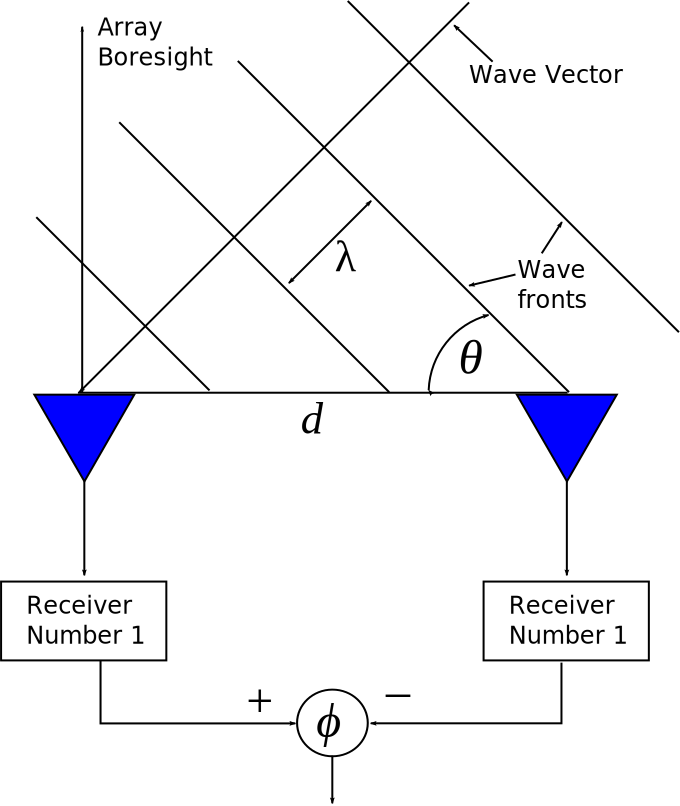
\includegraphics[width=0.4\textwidth]{lit_review/two_element_phase_df_model.pdf}
   \caption{Two-element phase interferometry. Note that as the element spacing (d) is more than half a wavelength there is ambiguity.}
   \label{fig:lit-two-element-phase}
\end{figure}

\subsection{Summary}
Amplitude based systems generally used for DF of cooperative emitters \cite{jenkins1991smallaperture}
This uses an antenna array. The antennas either have gain themselves or beam forming techniques are used to create beams with gains. Amplitude comparison techniques are in general simple to implement, but provide low resolution and low accuracy compared to phase methods due to their dependence on antenna beam pattern and their sensitivity to multipath. In practice, typical amplitude comparison systems have a DF RMS accuracy between \SI{3}{\degree} and \SI{10}{\degree}.

\section{Stuff from Schleher}
The simplest way to do DF is scan a narrow beam antenna. The position of the antenna which produces the highest output is the AoA. The antenna can be scanned physically by rotating it or electronically by a phased array. 
The down side of this approach is it cannot DF transients as it has a low POI. Well, POI as well as it needs time to scan around to figure out where the highest amplitude signal is.

Angular accuracy is:
\begin{equation}
  \Delta \theta = k \theta_B / \sqrt{SNR}
\end{equation}

Interferometer systems which use phase comparison for DF have a comparatively higher angular accuracy and rapid response which is good for transient detection. However, they impose stringent requirements on the phase matching for the RF chain which requires careful design, measurement and calibration. 

Selection of antenna spacing necessitates a trade off between angular accuracy and ambiguity. The further the elements are placed apart, the greater the accuracy, but the more ambiguity is introduced. It is well known that for a 2-element array, the lowest ambiguity which can be achieved is \SI{180}{\degree} which is when the elements are spaced half a wavelength apart. 
Of course, this \(\lambda/2\) is only valid for a single frequency. As soon as a different frequency needs to be received, the antennas will appear closer together or further apart, depending on whether the new frequency is higher or lower. As such, the specing is generally set by the highest frequency needed to be received, which puts an upper bound on the amount of ambiguity in the system. 

For a linear array, the array is often constructed with a long baseline (in the order of \(16\lambda\)) to provide high angular accuracy, and a short baseline \(\lambda/2\) to resolve the ambiguity introduced by the system. It must be noted that with a linear array, there is always an unresolvable \SI{180}{\degree} ambiguity, no matter how many elements are present.

DF can also be done via Doppler shift which involves rapidly switching which antenna is sampled in an array to simulate rapidly rotating the antenna. When the antenna is being switched toward the signal source, the received frequency will go up. When the sampled antenna is being switched away from the source, the frequency will go down. By seeing at which stage of the switching the frequency is increasing and at which stage it is decreasing, it can be determined where the source is.

TODO: insert summary table from page 384 here.

Geolocation is done by measuring AoA from multiple locations and then triangulating to ascertain the true location of the source. This is outside the scope of this project. This project seeks only to design an AoA system. Not a geolocation system. 

Probability of Intercept (POI) is a measure of the probability that the parameters of the EW receiving system match those of the target signal source at an instant in time. The key parameters are frequency and orientation. Frequency refers to whether the receiver is receiving on the frequency which is being transmitted. Orientation refers to whether the antennas of the receiver are pointed towards the signal source. 
For a \SI{100}{\percent} POI, the receiver needs to be wide open (as opposed to narrow-band scanning) and have omni directional antenna coverage. This \SI{100}{\percent} POI is essential to be able to intercept transient or impulsive signals.
